\section{Verification in the Presence of Faults}
\label{sec:analysisResults}
There are two main options for fault model analysis using the Safety Annex. The first option injects faults into the Lustre program based on the restrictions placed through the fault hypothesis. The Bounded Model Checker (BMC) engine used in JKind will find a {\em counterexample} to an invalid property. These counterexamples are returned to the user and include a trace of the system state that causes the violation. This includes any active faults that were part of that violation. The second option is used to generate minimal cut sets for the model. The details of minimal cut set generation can be found in Chapter~\ref{chap:mcsGen} and a full description of the analysis results for minimal cut set generation can be found there. 

\subsubsection{Counterexamples}
An important feature of a bounded temporal logic model checker is the ability to find counterexamples. When the model checker determines that a formula with a universal path quantifier (e.g., for all paths...) is false, it will find a computation path which demonstrates that the negation of the formula is true. Likewise when the model checker determines that an existential path quantifier is true (e.g., there exists a path...), it will find a computation path that demonstrates why the formula is true~\cite{clarke2018model}. 

The guarantees in an AGREE contract contain an implicit universal quantifier. Thus, if a guarantee states: $(a > b) \implies c$, this is translated as ``for all states, if $a > b$, then $c$." If this is invalid, the counterexample will include values within the constraints of the model for $a$, $b$, and $c$ such that $(a > b) \centernot \implies c$.

These counterexamples provide, in the nominal verification, insights into assumptions and guarantees for each component and how they may be strengthened to support correct behavior. In fault analysis, the counterexamples include active faults. Assuming that the nominal model (the model in the absence of faults) proves the specified properties, if verification in the presence of faults returns a counterexample, it is clear that an active fault caused the violation of the property. Insight into the state of the system when this occurs is invaluable to an analyst. This information can be used in the model-based safety assessment process to drive design changes. 

\subsubsection{Verification in the Presence of Faults: Max \textit{n} Analysis}
Using a max number of faults for the hypothesis, the user can constrain the number of simultaneously active faults in the model. The faults are added to the system subcomponents and a fault hypothesis statement is added to the component implementation. Given the constraint on the number of possible simultaneously active faults, the model checker attempts to prove the top level properties given these constraints. If this cannot be done, a counterexample is provided that shows which of the faults are active and which contracts are violated. We assume that the nominal model properties prove in the absence of faults.

The user can choose to perform either compositional or monolithic analysis using a max $n$ fault hypothesis. In compositional analysis, the analysis proceeds in a top down fashion. To prove the top level properties, the properties in the layer directly beneath the top level are used to perform the proof. The analysis proceeds in this manner. Users constrain the maximum number of faults within each layer of the model by specifying the maximum fault hypothesis statement to that layer. If any lower level property failed due to activation of faults, the property verification at the higher level can no longer be trusted because the higher level properties were proved based on the assumption that the direct sub-level contracts are valid. This form of analysis is helpful to see weaknesses in a given layer of the system. 

In monolithic analysis the layers of the model are flattened, which allows a direct correspondence between all faults in the model and their effects on the top level properties. As with compositional analysis, a counterexample shows these $n$ or less active faults. 

Returning to the PWR system example, we wish to see if the faults defined for the sensors contribute to a violation of the top level safety property (shut down occurs when and only when it should). The model has two distinct layers: top level with subsystems as subcomponents and leaf level with sensor subcomponents. If verification in the presence of faults is run compositionally with maximum 2 faults active, the results are as shown in Figure~\ref{fig:maxNPWRVerif}. 

\begin{figure}[h!]
	%\vspace{-0.1in}
	%\begin{center}
		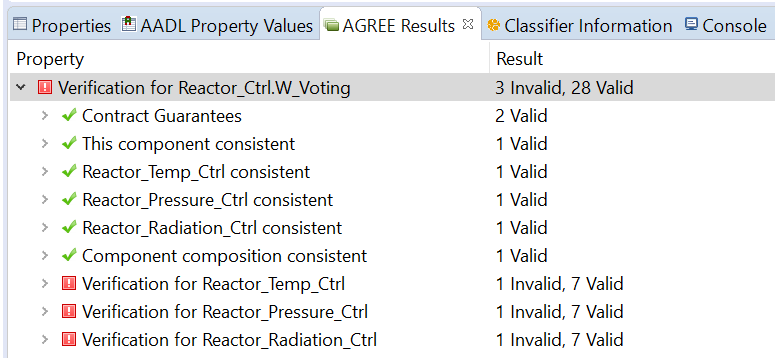
\includegraphics[width=0.8\textwidth]{images/maxNPWRVerif.png}
	%\end{center}
	%\vspace{-0.1in}
	\caption{PWR Verification with Maximum Two Faults Hypothesis}
	\label{fig:maxNPWRVerif}
\end{figure}

The top level verification passes because faults are not defined at that level. The leaf level verification, however, does not pass; the property at the subsystem level is violated. Selecting to view the counterexample, we see that two active faults on two sensors will violate the subsystem property. The counterexample spreadsheet view is shown in Figure~\ref{fig:maxNPWRVerifCoex}. 

\begin{figure}[h!]
	%\vspace{-0.1in}
	%\begin{center}
		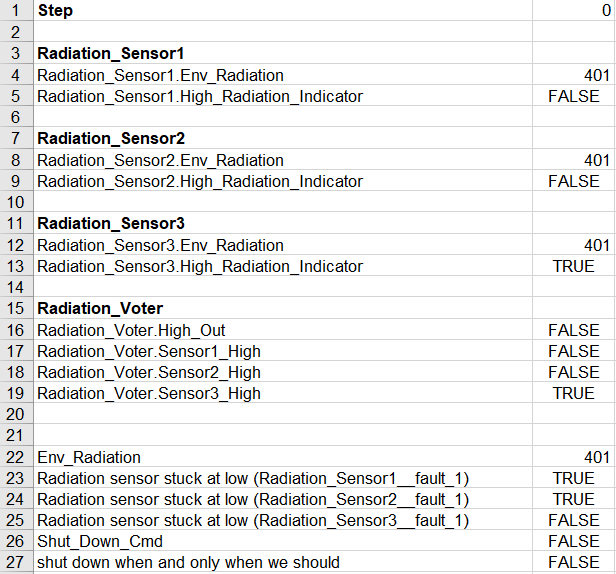
\includegraphics[width=0.6\textwidth]{images/maxNPWRVerifCoex.png}
	%\end{center}
	%\vspace{-0.1in}
	\caption{PWR Counterexample with Maximum Two-Faults Hypothesis}
	\label{fig:maxNPWRVerifCoex}
\end{figure}

A monolithic verification in the presence of faults will show that the top level safety property is violated; the subsystem guarantee directly supports the proof of the top level safety property. 

\subsubsection{Verification in the Presence of Faults: Probabilistic Analysis} 
Given a probabilistic fault hypothesis, this corresponds to performing analysis with the combinations of faults whose occurrence probability is less than the probability threshold. This is done by inserting assertions that allow those combinations in the Lustre code. If the model checker proves that the safety properties can be violated with any of those combinations, one of such combination will be shown in the counterexample. 

Probabilistic analysis done in this way must utilize the monolithic AGREE option. For compositional probabilistic analysis, see Chapter~\ref{chap:mcsGen} of this dissertation.

\begin{algorithm}[H]
	% \KwData{this text}
	% \KwResult{how to write algorithm with \LaTeX2e }
	$\mathcal{F} = \{\}$ : fault combinations above threshold \;
	$\mathcal{Q}$ : faults, $q_i$, arranged with probability high to low \;
	$\mathcal{R} = \mathcal{Q}$ , with $r \in \mathcal{R}$\;
	\While{$\mathcal{Q} \neq \{\} \land \mathcal{R} \neq \{\}$ }{
		$q =$ removeTopElement($\mathcal{Q}$) \;
		\For{$i=0:|\mathcal{R}|$}{
			$prob = q \times r_i$ \;
			\eIf{prob $<$ threshold}{
				removeTail($\mathcal{R}, j=i:|\mathcal{R}|$)\;
			}{
				add($\{q, r_i\}, \mathcal{Q}$)\;
				add($\{q, r_i\}, \mathcal{F}$)\;
			} % end if else
		} % end for
	} % end while
	\caption{Monolithic Probability Analysis}
	\label{alg:prob_monolithic}
\end{algorithm}

To perform this analysis, it is assumed that the non-hardware faults occur independently and possible combinations of faults are computed and passed to the Lustre model to be checked by the model checker. As seen in Algorithm 1, the computation first removes all faults from consideration that are too unlikely given the probability threshold. The remaining faults are arranged in a priority queue $\mathcal{Q}$ from high to low. Assuming independence in the set of faults, we take a fault with highest probability from the queue (step 5) and attempt to combine the remainder of the faults in $\mathcal{R}$ (step 7). If this combination is lower than the threshold (step 8), then we do not take into consideration this set of faults and instead remove the tail of the remaining faults in $\mathcal{R}$. 
 
In this calculation, we assume independence among the faults, but in the Safety Annex it is possible to define dependence between faults using a fault propagation statement. After fault combinations are computed using Algorithm~\ref{alg:prob_monolithic}, the triggered dependent HW faults are added to the combination as appropriate. 

In the PWR system, each sensor can fail with probability $1.0 \times 10^{-5}$ and the probabilistic threshold for the system safety property is given as $1.0 \times 10^{-9}$. Running monolithic verification in the presence of faults shows that given the voting mechanism, no faults will violate the safety property. By lowering the probabilistic threshold to $1.0 \times 10^{-10}$, the safety property is violated with two active faults on any sensor subsystem as shown in Figure~\ref{fig:probPWRVerif}.

\begin{figure}[h!]
	%\vspace{-0.1in}
	%\begin{center}
		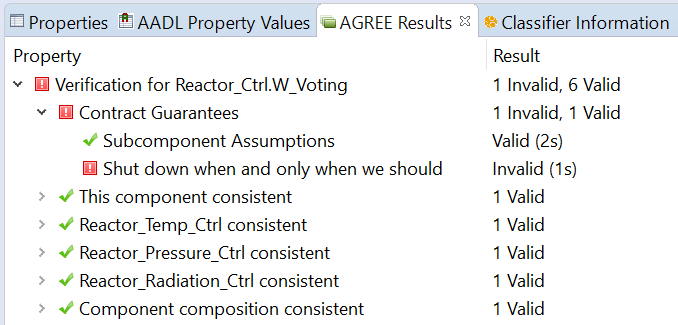
\includegraphics[width=0.8\textwidth]{images/probPWRVerif.png}
	%\end{center}
	%\vspace{-0.1in}
	\caption{PWR Verification with Probabilistic Hypothesis}
	\label{fig:probPWRVerif}
\end{figure}

Figure~\ref{fig:probPWRVerifCoex} shows a portion of the counterexample provided by the model checker for the probabilistic hypothesis of $1.0 \times 10^{-10}$. 

\begin{figure}[h!]
	%\vspace{-0.1in}
	%\begin{center}
		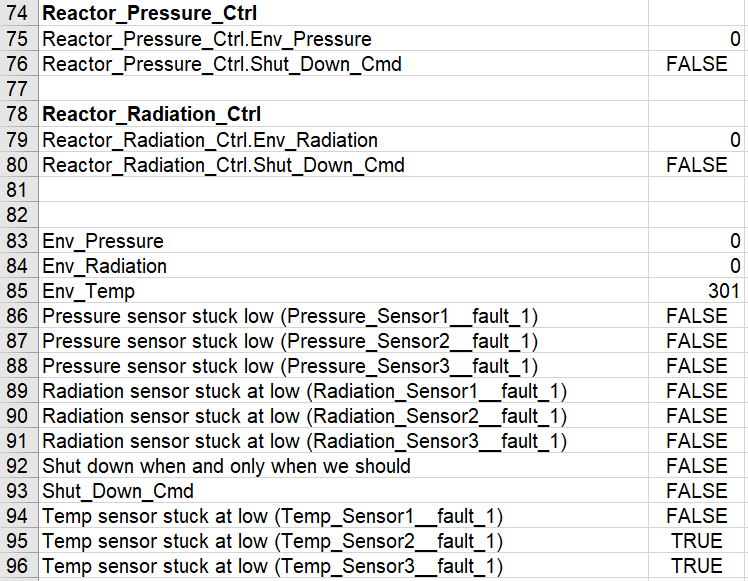
\includegraphics[width=0.6\textwidth]{images/probPWRVerifCoex.png}
	%\end{center}
	%\vspace{-0.1in}
	\caption{PWR Counterexample with Probabilistic Hypothesis}
	\label{fig:probPWRVerifCoex}
\end{figure}

The counterexample shows the active faults on the temperature subsystem: two faults are simultaneously active which violates the safety property. 

A benefit of utilizing the capabilities of counterexample generation is to ability for an analyst to view the dynamic behavior of a complex system and be able to understand the signal flow between behaviorally connected components. This aids in the design process when using model-based engineering methods and can greatly assist in design restructuring changes that may need to occur. It can be easy to see through counterexamples when a system is not resilient to a single fault, or when a combination of faults are sufficiently likely to occur together. Using these analysis capabilities support the objective to provide formal feedback to a safety engineer during the analysis of a complex critical system.

Up until this point, we have discussed modeling capabilities and counterexample generation using the safety annex for MBSA, but these counterexamples produce only a single path towards violation; in practice, safety analysts seek to find all minimal paths towards violation in terms of minimal cut sets. Given the analysis capabilities of a model checker in terms of proof cores -- the minimal set of model contracts required for a proof of the safety property -- we turn our attention towards leveraging this capability in terms of potentially active faults. 